\documentclass[tikz]{standalone}
\usepackage[sfdefault,light]{roboto}
\usetikzlibrary{shapes, arrows, positioning, fit, backgrounds}
\tikzset{every picture/.style={/utils/exec={\sffamily}}}
\definecolor{MyGreen}{HTML}{41B3A3}
\begin{document}
    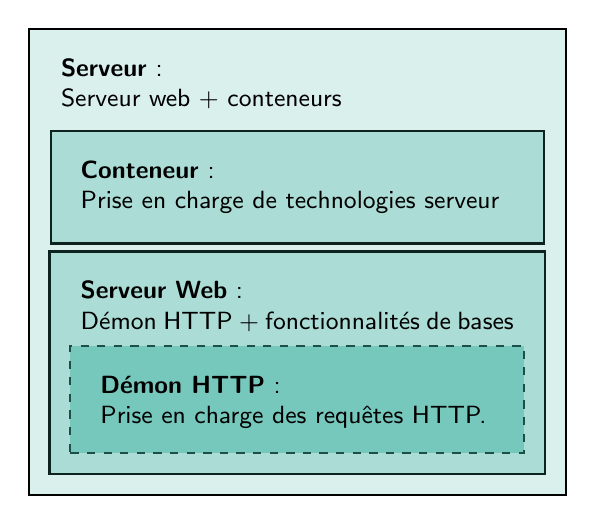
\begin{tikzpicture}[
			every node/.style={draw,rectangle,thick, font=\small},
			env/.style={draw,rectangle,thick,inner sep=0.25cm}
		]
		\node (http) [anchor=south west,draw=none] at (0,0) 
		{
            \begin{minipage}[t][.6cm]{5cm}
                \textbf{Démon HTTP} : \\
                Prise en charge des requêtes HTTP.
			\end{minipage}};
		\node (web) [above=0.3cm of http,draw=none] 
		{
            \begin{minipage}[t]{5.5cm}
                \textbf{Serveur Web} :\\
                Démon HTTP + fonctionnalités de bases
			\end{minipage}};
		\node (conteneur) [above=0.6cm of web,draw=none] 
		{
            \begin{minipage}[t]{5.5cm}
                \textbf{Conteneur} : \\
                Prise en charge de technologies serveur
			\end{minipage}};
		\node (appli) [above=0.4cm of conteneur,draw=none] 
		{
            \begin{minipage}[t]{6cm}
                \textbf{Serveur} :\\
                Serveur web + conteneurs
			\end{minipage}};
		\begin{scope}[on background layer]
			\node (envHttp) [env,fit=(http),fill opacity=0.5,fill=MyGreen,dashed] {};
			\node (envWeb) [env,fit=(web) (envHttp),fill opacity=0.3,fill=MyGreen] {};
			\node (envCont) [env,fit=(conteneur),fill opacity=0.3,fill=MyGreen] {};
			\node (envAppli) [env,fit=(appli) (envCont) (envWeb),fill opacity=0.2,fill=MyGreen] {};
		\end{scope}
	\end{tikzpicture}
\end{document}